\documentclass[11pt]{article}
\usepackage[margin=1in]{geometry}
\usepackage{booktabs}
\usepackage{array}
\usepackage{graphicx}
\usepackage{enumitem}
\usepackage[htt]{hyphenat}
\sloppy
\usepackage[colorlinks=true,urlcolor=blue,linkcolor=black]{hyperref}

\title{Wearables and Habits: Synthetic Control Estimates\\\large Issue \#9}
\date{4 October 2026}
\author{}

\begin{document}
\maketitle

\section{Summary}
Exploratory unit-level synthetic control of first wearable purchase on running-related purchases, as an alternative to the staggered DiD of \#7 (which fails on pre-trends). \textbf{Balanced panel only}, and each adopter's synthetic twin is matched on outcome history, purchase intensity, category mix and survey demographics (Section~\ref{sec:design}).
\begin{itemize}[nosep]
\item \textbf{Running-related purchasing rises modestly, but so does everything else.} Post ATT (quarters 1--$L$): running-related $+0.046$ (0.017) with $L=8$ (113 adopters) and $+0.039$ (0.013) with $L=6$ (242); running shoes $+0.016$ (0.012) and $+0.013$ (0.008); supplements $+0.066$ (0.025) and $+0.050$ (0.017); fitness gear and medication are within about 1.5 SE of zero.
\item \textbf{Non-running outcomes move too.} Books $+0.042$ (0.023) / $+0.040$ (0.016), grocery $+0.040$ / $+0.010$, pet $+0.035$ / $+0.020$, and total purchases $\ln(1+n)$ $+0.264$ (0.054) / $+0.205$ (0.040). Adopters buy more overall than their twins after adoption, and the running-related gain is of the same size as the books placebo, so it cannot be attributed to running specifically.
\item \textbf{Pre-fit and balance.} Pre-period gaps are about zero (Figures~\ref{fig:main}, \ref{fig:plac}), so the pre-trend problem of \#7 is absorbed by the twin. Category shares and most demographics are close to the adopters' (Table~\ref{tab:bal}); the exceptions are pre-period $\ln$ spend (8.22 vs 8.07 synthetic) and income band (2.89 vs 2.72).
\item \textbf{Pseudo-adopter placebo} (random never-treated users given real adoption dates) is about zero for nearly all outcomes (largest: pet $+0.034$ at $L=8$, supplements $-0.027$ at $L=6$).
\item \textbf{Relation to earlier runs and \#7.} A preliminary unbalanced-panel run (outcome-only matching, 288 adopters; kept in \texttt{synth\_summary*.csv}) gave larger gaps (running-related $+0.070$). The DiD of \#7 gave small \emph{negative} estimates, so the methods still disagree in sign. A plausible common driver is selection of adopters on a purchase in $e=0$ and on $\geq$12 months of later activity, which donors are not selected on; this predicts positive gaps for all outcomes. Not tested.
\end{itemize}

\section{Design}\label{sec:design}
\begin{itemize}[nosep]
\item \textbf{Balanced sample:} ``clean'' sample users observed in every quarter 2018Q1--2022Q4 (2{,}764 users). Adopters must have the full window $g-L,\dots,g+L$ inside 2018Q1--2022Q4: $L=8$ gives adoption in 2020 (113 adopters), $L=6$ in 2019Q3--2021Q2 (242). Donors: balanced never-treated users (2{,}392). No unobserved quarters, so donors are never dropped in the post-period.
\item \textbf{What is matched} (donors and adopter use the same calendar pre-window $g-L,\dots,g-1$), four blocks, each column standardized by the donor-pool SD and scaled so a block's total weight is:
\begin{enumerate}[nosep]
\item weight 2: the studied outcome (any purchase in the quarter) in each pre-quarter;
\item weight 1: $\ln(1+\mathrm{purchases})$ in each pre-quarter (omitted when it is the outcome);
\item weight 1: pre-window category mix, the share of purchases in running-related, fitness gear, supplements, medication, pet, books, gift cards, cables/batteries, cleaning and grocery, plus $\ln(1+\mathrm{total spend})$;
\item weight 1: survey demographics: age band, income band, household size, female, college, white, diabetes, smoker, alcohol, and a survey-missing flag (mean-imputed as in \#7).
\end{enumerate}
\item \textbf{Weights:} non-negative, sum to one, least squares over the 150 nearest donors (distance on the same standardized predictors). With four blocks the fit is a compromise, so pre-RMSE on the outcome is larger than with outcome-only matching.
\item \textbf{Effects:} gap = adopter minus synthetic, $e=-L,\dots,L$ ($e=0$ the adoption quarter); ATT$_e$ = mean over adopters; SE = cross-adopter SD$/\sqrt n$ (ignores weight estimation error). Post ATT = mean over $e=1,\dots,L$. Placebo: as many never-treated users as adopters get randomly drawn real adoption quarters and are run against the remaining donors.
\item Code: \texttt{code/scripts/synth\_control\_balanced.py} (argument $L$) and \texttt{synth\_control\_balanced\_figs.py}.
\end{itemize}

\section{Results}
\begin{table}[h]\centering\small
\caption{Balanced synthetic control, $L=8$ (113 adopters). Pre RMSE = RMS adopter-minus-synthetic gap in the pre-period / RMS outcome level.}
\begin{tabular}{lrrrr}
\toprule
Outcome & Post ATT (SE) & Placebo (SE) & N & Pre RMSE / level \\
\midrule
Running shoe & 0.016 (0.012) & 0.001 (0.005) & 113 & 0.017 / 0.102 \\
Running-related (keyword) & 0.046 (0.017) & 0.001 (0.014) & 113 & 0.050 / 0.278 \\
Fitness gear & 0.015 (0.013) & 0.004 (0.013) & 113 & 0.027 / 0.190 \\
Supplements & 0.066 (0.025) & 0.017 (0.022) & 113 & 0.079 / 0.366 \\
Medication & 0.034 (0.020) & 0.011 (0.018) & 113 & 0.034 / 0.208 \\
PLACEBO: pet & 0.035 (0.022) & 0.034 (0.023) & 113 & 0.074 / 0.401 \\
PLACEBO: books & 0.042 (0.023) & -0.001 (0.021) & 113 & 0.111 / 0.588 \\
PLACEBO: grocery/food & 0.040 (0.022) & 0.011 (0.023) & 113 & 0.050 / 0.266 \\
General: ln(1+\#purchases) & 0.264 (0.054) & -0.003 (0.062) & 113 & 0.280 / 2.939 \\
\bottomrule
\end{tabular}
\end{table}
\begin{table}[h]\centering\small
\caption{Balanced synthetic control, $L=6$ (242 adopters).}
\begin{tabular}{lrrrr}
\toprule
Outcome & Post ATT (SE) & Placebo (SE) & N & Pre RMSE / level \\
\midrule
Running shoe & 0.013 (0.008) & -0.009 (0.005) & 242 & 0.007 / 0.080 \\
Running-related (keyword) & 0.039 (0.013) & 0.000 (0.011) & 242 & 0.030 / 0.253 \\
Fitness gear & 0.019 (0.010) & 0.010 (0.009) & 242 & 0.017 / 0.174 \\
Supplements & 0.050 (0.017) & -0.027 (0.015) & 242 & 0.053 / 0.365 \\
Medication & -0.007 (0.013) & 0.006 (0.014) & 242 & 0.023 / 0.212 \\
PLACEBO: pet & 0.020 (0.015) & -0.005 (0.018) & 242 & 0.048 / 0.378 \\
PLACEBO: books & 0.040 (0.016) & 0.015 (0.016) & 242 & 0.087 / 0.570 \\
PLACEBO: grocery/food & 0.010 (0.017) & 0.020 (0.017) & 242 & 0.035 / 0.274 \\
General: ln(1+\#purchases) & 0.205 (0.040) & 0.008 (0.043) & 242 & 0.230 / 3.016 \\
\bottomrule
\end{tabular}
\end{table}
\begin{figure}[h]\centering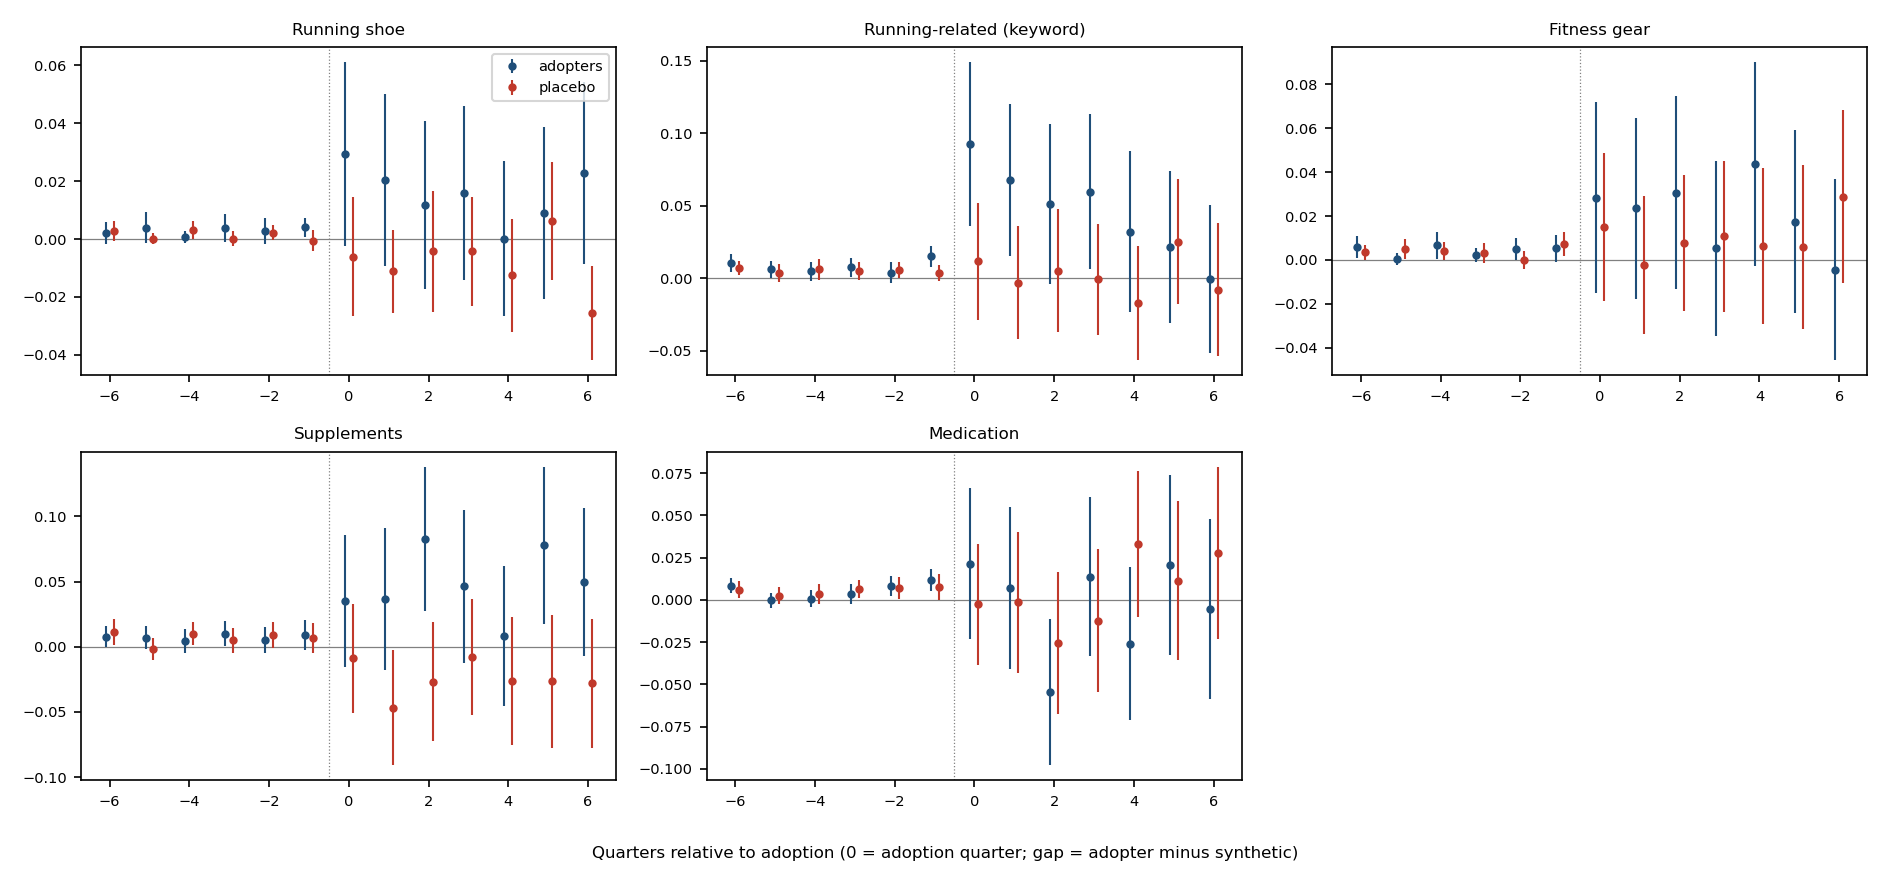
\includegraphics[width=\textwidth]{../code/analysis/outputs/synth_bal_es_main_L6.png}
\caption{Event-study gaps, main outcomes, $L=6$ (blue adopters, red pseudo-adopter placebo; 95\% CIs). $L=8$: \texttt{synth\_bal\_es\_main\_L8.png}.}\label{fig:main}\end{figure}
\begin{figure}[h]\centering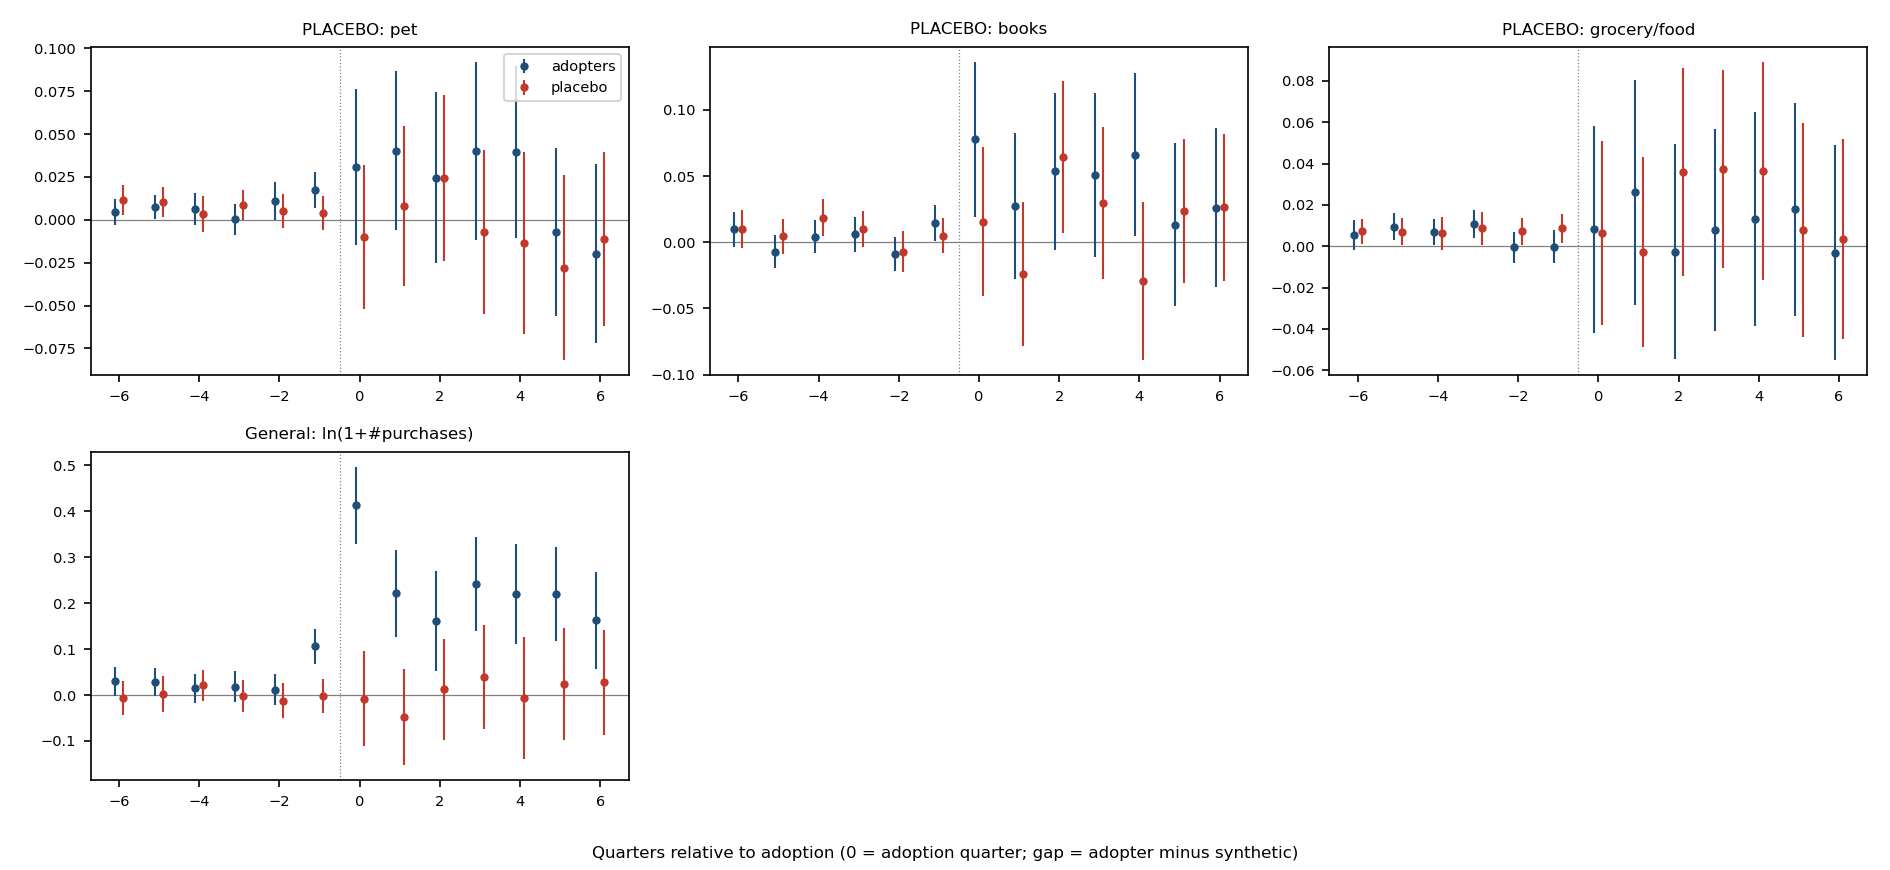
\includegraphics[width=\textwidth]{../code/analysis/outputs/synth_bal_es_placebo_L6.png}
\caption{Same, placebo and general-intensity outcomes.}\label{fig:plac}\end{figure}
\begin{table}[h]\centering\small
\caption{Covariate balance, $L=8$, running-related fit: average adopter, synthetic twin and raw donor pool.}\label{tab:bal}
\begin{tabular}{lrrr}
\toprule
Variable & Adopters & Synthetic & Donor pool \\
\midrule
share: run\_any & 0.009 & 0.009 & 0.006 \\
share: fit\_gear & 0.004 & 0.004 & 0.004 \\
share: supp & 0.017 & 0.018 & 0.019 \\
share: med & 0.006 & 0.006 & 0.006 \\
share: pet & 0.028 & 0.027 & 0.023 \\
share: book & 0.066 & 0.067 & 0.071 \\
share: giftcard & 0.015 & 0.019 & 0.024 \\
share: cable & 0.024 & 0.024 & 0.023 \\
share: cleaning & 0.004 & 0.004 & 0.004 \\
share: grocery & 0.012 & 0.015 & 0.014 \\
ln spend (pre) & 8.216 & 8.069 & 7.500 \\
age & 1.841 & 1.950 & 1.888 \\
inc & 2.885 & 2.720 & 2.321 \\
hh & 2.619 & 2.547 & 2.399 \\
female & 0.513 & 0.534 & 0.531 \\
college & 0.743 & 0.715 & 0.659 \\
white & 0.867 & 0.863 & 0.801 \\
diab & 0.081 & 0.096 & 0.126 \\
smoke & 0.090 & 0.104 & 0.127 \\
alc & 0.438 & 0.470 & 0.460 \\
svy\_miss & 0.009 & 0.005 & 0.018 \\
\bottomrule
\end{tabular}
\end{table}

\section{Caveats and follow-ups}
\begin{itemize}[nosep]
\item Balanced sample means long-lived, early-start users and adopters in a narrow calendar window (2020 for $L=8$), so results are not comparable to \#7's 447.
\item Follow-ups (not done): hold-out pre-period fit; synthetic DiD / augmented SC; pseudo-adopters selected on an $e=0$ purchase; not-yet-treated donors; tuning predictor block weights.
\end{itemize}
\end{document}
